\documentclass{standalone}
\usepackage{pgfplots}

\usepgfplotslibrary{patchplots}
\pgfplotsset{compat=1.13}

\begin{document}

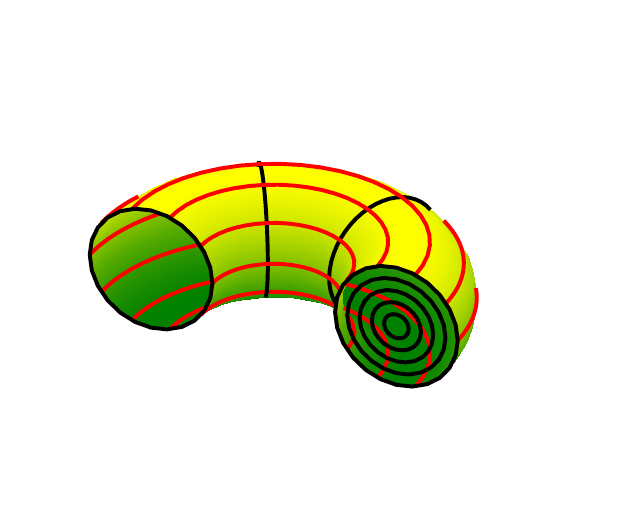
\begin{tikzpicture}
\def\innerRadius{1}
\def\outerRadius{2}
    \begin{axis}[
      axis equal,
      axis line style={draw=none},
      tick style={draw=none},
      xticklabels={,,},
      yticklabels={,,},
      zticklabels={,,}
    ]
    \addplot3[surf,
    colormap/greenyellow,
    shader=interp,
    samples=20, samples y = 20,
    domain=0:2*pi,y domain=0:pi,
    z buffer=sort]
    ({(\outerRadius+\innerRadius*cos(deg(x)))*cos(deg(y))}, 
    {(\outerRadius+\innerRadius*cos(deg(x)))*sin(deg(y))}, 
    {\innerRadius*sin(deg(x))});
    
    \addplot3[domain=2.6:pi, line width=0.5mm, mark=none, color=red, samples y=0]
         ({(\outerRadius+\innerRadius*cos(deg(pi*1.4)))*cos(deg(x))}, 
	  {(\outerRadius+\innerRadius*cos(deg(pi*1.4)))*sin(deg(x))}, 
	  {\innerRadius*sin(deg(pi*1.4))});
    
    \addplot3[domain=2.4:pi, line width=0.5mm, mark=none, color=red, samples y=0]
         ({(\outerRadius+\innerRadius*cos(deg(pi*1.6)))*cos(deg(x))}, 
	  {(\outerRadius+\innerRadius*cos(deg(pi*1.6)))*sin(deg(x))}, 
	  {\innerRadius*sin(deg(pi*1.6))});
    
    \addplot3[domain=2.4:pi, line width=0.5mm, mark=none, color=red, samples y=0]
         ({(\outerRadius+\innerRadius*cos(deg(pi*1.8)))*cos(deg(x))}, 
	  {(\outerRadius+\innerRadius*cos(deg(pi*1.8)))*sin(deg(x))}, 
	  {\innerRadius*sin(deg(pi*1.8))});
  
    \addplot3[domain=1.1:pi, line width=0.5mm, mark=none, color=red, samples y=0]
         ({(\outerRadius+\innerRadius*cos(deg(pi*1.2)))*cos(deg(x))}, 
	  {(\outerRadius+\innerRadius*cos(deg(pi*1.2)))*sin(deg(x))}, 
	  {\innerRadius*sin(deg(pi*1.2))});
    
  % Z
    
    \addplot3[domain=0.6:pi*1.15, line width=0.5mm, mark=none, color=black, samples y=0]
         ({(\outerRadius+\innerRadius*cos(deg(x)))*cos(deg(pi/3))}, 
	  {(\outerRadius+\innerRadius*cos(deg(x)))*sin(deg(pi/3))}, 
	  {\innerRadius*sin(deg(x))});
    
    \addplot3[domain=0.7:pi*1.3, line width=0.5mm, mark=none, color=black, samples y=0]
         ({(\outerRadius+\innerRadius*cos(deg(x)))*cos(deg(2*pi/3))}, 
	  {(\outerRadius+\innerRadius*cos(deg(x)))*sin(deg(2*pi/3))}, 
	  {\innerRadius*sin(deg(x))});
    
    \addplot3[domain=0:0.53, line width=0.5mm, mark=none, color=red, samples y=0]
         ({(\outerRadius+\innerRadius)*cos(deg(x))}, 
	  {(\outerRadius+\innerRadius)*sin(deg(x))}, 
	  {0});
	 
    \addplot3[domain=0:0.9, line width=0.5mm, mark=none, color=red, samples y=0]
         ({(\outerRadius+\innerRadius*cos(deg(pi/5)))*cos(deg(x))}, 
	  {(\outerRadius+\innerRadius*cos(deg(pi/5)))*sin(deg(x))}, 
	  {\innerRadius*sin(deg(pi/5))});

    \addplot3[domain=0:0.9, line width=0.5mm, mark=none, color=red, samples y=0]
         ({(\outerRadius+\innerRadius*cos(deg(pi*1.2)))*cos(deg(x))}, 
	  {(\outerRadius+\innerRadius*cos(deg(pi*1.2)))*sin(deg(x))}, 
	  {\innerRadius*sin(deg(pi*1.2))});
    
    \addplot3[domain=0:1.35, line width=0.5mm, mark=none, color=red, samples y=0]
         ({(\outerRadius+\innerRadius*cos(deg(pi*1.4)))*cos(deg(x))}, 
	  {(\outerRadius+\innerRadius*cos(deg(pi*1.4)))*sin(deg(x))}, 
	  {\innerRadius*sin(deg(pi*1.4))});
    
    \addplot3[domain=0:1.53, line width=0.5mm, mark=none, color=red, samples y=0]
         ({(\outerRadius+\innerRadius*cos(deg(pi*1.6)))*cos(deg(x))}, 
	  {(\outerRadius+\innerRadius*cos(deg(pi*1.6)))*sin(deg(x))}, 
	  {\innerRadius*sin(deg(pi*1.6))});
	  
    \foreach \r in {0.2,0.4,...,0.9}
    {
     \addplot3[domain=0:pi*2, line width=0.5mm, mark=none, color=black, samples y=0]
         ({(\outerRadius+\r*cos(deg(x)))}, 
	  {0}, 
	  {\r*sin(deg(x))});
    }
    
    \addplot3[domain=2.6:pi, line width=0.5mm, mark=none, color=red, samples y=0]
         ({(\outerRadius+\innerRadius)*cos(deg(x))}, 
	  {(\outerRadius+\innerRadius)*sin(deg(x))}, 
	  {0});
    
    
    \addplot3[domain=2.8:pi, line width=0.5mm, mark=none, color=red, samples y=0]
         ({(\outerRadius+\innerRadius*cos(deg(pi/5)))*cos(deg(x))}, 
	  {(\outerRadius+\innerRadius*cos(deg(pi/5)))*sin(deg(x))}, 
	  {\innerRadius*sin(deg(pi/5))});

    \foreach \q in {0.4,0.6,0.8}
    {
     \pgfmathsetmacro\theta{\q*pi}
     \addplot3[domain=0:pi, line width=0.5mm, mark=none, color=red, samples y=0]
         ({(\outerRadius+\innerRadius*cos(deg(\theta)))*cos(deg(x))}, 
	  {(\outerRadius+\innerRadius*cos(deg(\theta)))*sin(deg(x))}, 
	  {\innerRadius*sin(deg(\theta))});
    }
    
    \addplot3[domain=0.6:pi, line width=0.5mm, mark=none, color=red, samples y=0]
         ({(\outerRadius+\innerRadius*cos(deg(pi)))*cos(deg(x))}, 
	  {(\outerRadius+\innerRadius*cos(deg(pi)))*sin(deg(x))}, 
	  {\innerRadius*sin(deg(pi))});
    
    \addplot3[domain=0:2*pi, line width=0.5mm, mark=none, color=black, samples y=0]
         ({(\outerRadius+\innerRadius*cos(deg(x)))}, 
	  {0}, 
	  {\innerRadius*sin(deg(x))});
	  
    \addplot3[domain=0:2*pi, line width=0.5mm, mark=none, color=black, samples y=0]
         ({-(\outerRadius+\innerRadius*cos(deg(x)))}, 
	  {0}, 
	  {\innerRadius*sin(deg(x))});
    \end{axis}
\end{tikzpicture}

\end{document}